\documentclass[addpoints,answers]{exam}
\usepackage[utf8]{inputenc}
\usepackage{amsmath}
\usepackage{amsfonts}
\usepackage{mathrsfs}

\usepackage{pgfplots}
\pgfplotsset{compat=newest}

\usepgfplotslibrary{polar}

\boxedpoints
\pointpoints{punto}{puntos}
\vqword{Pregunta}
\vpgword{Página}
\vpword{Puntos}
\vsword{Nota}
\vtword{Total}
\renewcommand{\solutiontitle}{\noindent\textbf{Respuesta:}\enspace}

\begin{document}

\header{TEL224}{Respuestas del primer examen (versión a)}{Viernes 13/03/2015}
\headrule

\title{Respuestas del primer examen (versión a) - TEL224}
\date{Viernes 13/03/2015}
\maketitle

\section*{Teoría}

\begin{questions}
\question[5]
Diseñe una señal discreta exponencial que no converja.

\begin{solution}
$$x[n] = 2^n u[n],\quad \forall n \in \mathbb{N}$$
\end{solution}

\question[5]
Defina y ejemplifique una FIR.

\begin{solution}
FIR significa "Finite-duration Impulse Response". Un sistema FIR es un sistema con respuesta al impulso de duración finita. El sistema siguiente es un sistema FIR:

$$h[n] = 2\delta[n]$$
\end{solution}

\question[5]
¿Qué es lo que sucede cuando una exponencial compleja (autofunción) atraviese un SLIT?

\begin{solution}
La salida de un SLIT atravesado por una exponencial compleja \(x[n] = e^{j\omega n}\) es la misma exponencial compleja multiplicada por el autovalor \(H\left(e^{j\omega}\right)\), o sea la respuesta en frecuencia del SLIT en la frecuencia \(\omega\):

$$
y[n] = H\left(e^{j\omega}\right) e^{j\omega n}
$$

con

$$
H\left(e^{j\omega}\right) = \sum_{k=-\infty}^{\infty} h[k] e^{-j\omega k}
$$
\end{solution}

\question[5]
Dibujar la región de convergencia de la transformada Z de una señal limitada por la derecha con un único polo en \(z=j\)

\begin{solution}
La región de convergencia de la transformada Z de una señal limitada por la derecha es el disco de rayo igual al módulo del polo menor. En este caso, existe un único polo, de módulo igual a \(1\), así que la región de convergencia esta definida por el disco \(|z| < 1\).

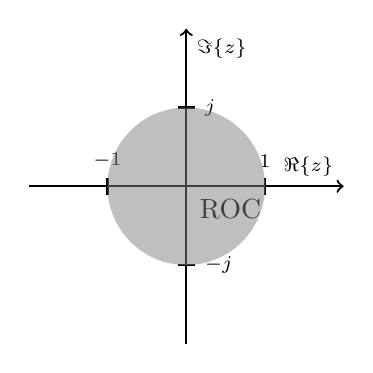
\begin{tikzpicture}
	\begin{scope}[thick,font=\scriptsize]
		% Axes:
		% Are simply drawn using line with the `->` option to make them arrows:
		% The main labels of the axes can be places using `node`s:
		\draw [->] (-2,0) -- (2,0) node [above left]  {$\Re\{z\}$};
		\draw [->] (0,-2) -- (0,2) node [below right] {$\Im\{z\}$};

		\draw (-1,-3pt) -- (-1,3pt)   node [above] {$-1$};
		\draw (1,-3pt) -- (1,3pt)   node [above] {$1$};
		\draw (-3pt,-1) -- (3pt,-1)   node [right] {$-j$};
		\draw (-3pt,1) -- (3pt,1)   node [right] {$j$};

	\end{scope}

	% The circle is drawn with `(x,y) circle (radius)`
	% You can draw the outer border and fill the inner area differently.
	% Here I use gray, semitransparent filling to not cover the axes below the circle
	\path [draw=none,fill=gray,semitransparent] (0,0) circle (1);

	% Place the text into the circle:
	\node [below right,darkgray] at (+0.05,-0.05) {ROC};
\end{tikzpicture}

\end{solution}

\question[5]
Dada la siguiente señal \(x[n]\), dibuje \(x[-(n-2)]\).

\begin{tikzpicture}
	\begin{axis}[
		axis x line=middle,
		axis y line=left,
		xtick={0,...,7},
		ytick={0,0.5,1},
		xmax=7.5, xmin=-0.5,
		ymax=1.1, ymin=-0.1
		]
		\addplot+[ycomb] plot coordinates
			{(0,0) (1,0) (2,0) (3,1) (4,1) (5,0.5) (6,0.5) (7,0)};
	\end{axis}
\end{tikzpicture}

\begin{solution}

Los únicos valores diferentes de cero son para \(n = 3, ...,6\), se transforman de la manera siguiente:

\begin{itemize}
	\item \(x[3] = 1\) se vuelve \(x[-1] = 1\)
	\item \(x[4] = 1\) se vuelve \(x[-2] = 1\)
	\item \(x[5] = 0.5\) se vuelve \(x[-3] = 0.5\)
	\item \(x[6] = 0.5\) se vuelve \(x[-4] = 0.5\)
\end{itemize}

\begin{tikzpicture}
	\begin{axis}[
		axis x line=middle,
		axis y line=left,
		xtick={-5,...,2},
		ytick={0,0.5,1},
		xmax=2.5, xmin=-5.5,
		ymax=1.1, ymin=-0.1
		]
		\addplot+[ycomb] plot coordinates
			{(-5,0) (-4,0.5) (-3,0.5) (-2,1) (-1,1) (0,0) (1,0) (2,0)};
	\end{axis}
\end{tikzpicture}

\end{solution}

\question[5]
Si la entrada del sistema es: \(x[n] = u[n]\) y su respuesta al impulso es: \(h[n] = \frac{1}{4}^{n-1} u[n-1]\), encuentre su salida. Recuerde: \(y[n] = x[n] * h[n]\)

\begin{solution}
\[
\begin{array}{ll}
	y[n]	&= x[n] * h[n] \\
			&= \sum_{k=-\infty}^{\infty}x[k]h[n-k] \\
			&= \sum_{k=0}^{\infty}h[n-k], \quad \text{porque } x[n]=0 \quad \forall n<0 \text{ y } x[n]=1 \quad \forall n \geq 0 \\
			&= \sum_{k=0}^{\infty}\frac{1}{4}^{n-k-1} u[n-k-1] \\
			&= \sum_{k=0}^{n-1}\frac{1}{4}^{n-k-1}, \quad \text{porque } u[n-k-1]=1 \quad \forall n-k-1 \geq 0 \text{ o sea  } k \leq n-1 \\
			&= \sum_{l=0}^{n-1}\frac{1}{4}^{l}, \quad \text{haciendo el cambio de variable } l=n-k-1 \\
			&= \frac{1-\left(\frac{1}{4}\right)^n}{1-\frac{1}{4}}, \quad \forall n \\
	y[n]	&= \frac{4}{3}\left(1-\left(\frac{1}{4}\right)^n\right), \quad \forall n
\end{array}
\]
\end{solution}


\question[10]
Encuentre la transformada Z unilateral de la señal: \(y[n] = 5 x[n-2] - x[n]\).

\begin{solution}
\[
\begin{array}{ll}
	\mathscr{Y}(z)	&= \sum_{n=0}^{\infty} \left(5 x[n-2] - x[n]\right)z^{-n} \\
					&= 5 \sum_{n=0}^{\infty} x[n-2] z^{-n} - \sum_{n=0}^{\infty} x[n] z^{-n} \\
					&= 5 \left( x[-2] + x[-1] z^{-1} + \sum_{n=2}^{\infty} x[n-2] z^{-n} \right) - \mathscr{X}(z) \\
					&= 5 \left( x[-2] + x[-1] z^{-1} + z^{-2} \sum_{n=2}^{\infty} x[n-2] z^{-(n-2)} \right) - \mathscr{X}(z) \\
					&= 5 \left( x[-2] + x[-1] z^{-1} + z^{-2} \sum_{n=0}^{\infty} x[n] z^{-n} \right) - \mathscr{X}(z) \\
					&= 5 \left( x[-2] + x[-1] z^{-1} + z^{-2} \mathscr{X}(z) \right) - \mathscr{X}(z) \\
					&= 5 x[-2] + 5 x[-1] z^{-1} + \left(5 z^{-2} -1 \right) \mathscr{X}(z)
\end{array}
\]
\end{solution}

\question
Del siguiente sistema: \(y[n] = x[n] - x[n-1]\), siendo \(x[n]\) la entrada y \(y[n]\) la salida:

\begin{parts}

\part[5]
Demuestre que es un sistema lineal invariante en el tiempo.

\begin{solution}
Mostremos que es un sistema lineal:

\[\begin{array}{ll}
T\left\{a x_1[n]+bx_2[n]\right\} &= \left(a x_1[n]+bx_2[n]\right) - \left(a x_1[n-1]+bx_2[n-1]\right) \\
&= a \left( x_1[n]-x_1[n-1]\right) + b \left( x_2[n]-x_2[n-1]\right) \\
&= a T\left\{x_1[n]\right\} + b T\left\{x_2[n]\right\}
\end{array}\]

Mostremos que es invariante en el tiempo. Si \(x_1[n] = x_[n-n_0]\),

\[\begin{array}{ll}
T\left\{x_1[n]\right\} &= x_1[n] - x_1[n-1] \\
&= x[n-n_0] - x[n-n_0-1] \\
&= T\left\{x[n-n_0]\right\}
\end{array}\]

\end{solution}

\part[5] 
Obtener \(h[n]\) y \(H\left(e^{j\omega}\right)\).

\begin{solution}

\[\begin{array}{ll}
h[n] &= T\left\{\delta[n]\right\} \\
&= \delta[n] - \delta[n-1]
\end{array}\]

\[\begin{array}{ll}
H\left(e^{j \omega}\right) &= \mathcal{F}\left\{\delta[n]-\delta[n-1]\right\} \\
&= 1 - e^{-j\omega} \\
&= e^{-\frac{j\omega}{2}} \left(e^{\frac{j\omega}{2}} - e^{-\frac{j\omega}{2}}\right) \\
&= 2j \sin\left(\frac{\omega}{2}\right) e^{-\frac{j\omega}{2}} \\
&= 2 \sin\left(\frac{\omega}{2}\right) e^{\frac{j(\pi - \omega)}{2}}
\end{array}\]

\end{solution}

\part[5] 
\(\left|H\left(e^{j\omega}\right)\right|\) y \(\angle H\left(e^{j\omega}\right)\).

\begin{solution}

El módulo es:

\[\begin{array}{ll}
\left|H\left(e^{j \omega}\right)\right| &= \left|2 \sin\left(\frac{\omega}{2}\right) e^{\frac{j(\pi - \omega)}{2}}\right| \\
&= 2 \left| \sin\left(\frac{\omega}{2}\right)\right|
\end{array}\]

La fase es:

\[\begin{array}{ll}
\angle H\left(e^{j \omega}\right) &= \angle 2 \sin\left(\frac{\omega}{2}\right) e^{\frac{j(\pi - \omega)}{2}} \\
&= \frac{\pi - \omega}{2}
\end{array}\]

\end{solution}

\part[5]

Obtener \(h_i[n]\) tal que \(h_i[n] * h[n] = \delta[n]\).

\begin{solution}
\[\begin{array}{ll}
h_i[n] * h[n] &= \sum_{k=-\infty}^{\infty} h_i[k] h[n-k] \\
&= \sum_{k=-\infty}^{\infty} h_i[k] \left(\delta[n-k] - \delta[n-k-1]\right) \\
&= h_i[n] - h_i[n-1]
\end{array}\]

Para que \(h_i[n] * h[n] = h_i[n] - h_i[n-1] = \delta[n]\), es necesario que:

\[
\left\{\begin{array}{ll}
h_i[n]-h_i[n-1] = 0, \quad \forall n < 0 \\
h_i[n]-h_i[n-1] = 1, \quad n=0 \\
h_i[n]-h_i[n-1] = 0, \quad \forall n > 0 \\
\end{array}\right.
\iff
\left\{\begin{array}{ll}
h_i[n] = h_i[n-1], \quad \forall n < 0 \\
h_i[0] = 1 + h_i[-1], \quad n=0 \\
h_i[n] = h_i[n-1], \quad \forall n > 0 \\
\end{array}\right.
\]

Esta relación esta verificada para todas las señales \(h_i[n] = A + u[n], \quad \forall A \in \mathbb{C}\)
\end{solution}

\end{parts}

\question
Si la entrada \(x[n]\) de un SLIT es \(x[n] = u[n]\), la salida es: \(y[n] = \left(\frac{1}{2}\right)^{n-1}u[n+1]\).

\begin{parts}
\part[5]
Hallar \(H(z)\) y su diagrama polo-cero.

\begin{solution}
\[X(z) = \frac{1}{1-z^{-1}}, \quad |z|>1\]
\[Y(z) = \frac{4z}{1-\frac{1}{2}z^{-1}}, \quad |z|> \frac{1}{2}\]

Entonces la función de transferencia es:
\[\begin{array}{ll}
H(z) &= \frac{Y(z)}{X(z)}, \quad |z|> \frac{1}{2} \\
&= \frac{4z\left(1-z^{-1}\right)}{1-\frac{1}{2}z^{-1}} , \quad |z|> \frac{1}{2} \\
&= \frac{4z\left(z-1\right)}{z-\frac{1}{2}} , \quad |z|> \frac{1}{2}
\end{array}\]

Su diagrama polo-cero es el siguiente:

\begin{tikzpicture}
\begin{polaraxis}[enlargelimits=false,
ytick={1},
yticklabels={},
xtick={0,90,...,360},
every outer x axis line/.append style={transparent},
every outer y axis line/.append style={transparent},
xticklabels={0,
$\frac{\pi}{2}$,
$\pi$,
$\frac{3\pi}{2}$},
]
    \addplot [
        mark=o,
        only marks
    ] coordinates {(0,0) (0,1)};
    \addplot [
        mark=x,
        only marks
    ] coordinates {(0,0.5)};

\end{polaraxis}
\end{tikzpicture}

\end{solution}

\part[5]
Obtener la respuesta al impulso: \(h[n]\):

\begin{solution}
\[\begin{array}{ll}
H(z) &= \frac{4z\left(1-z^{-1}\right)}{1-\frac{1}{2}z^{-1}} , \quad |z|> \frac{1}{2} \\
&= \frac{4z}{1-\frac{1}{2}z^{-1}} - \frac{4}{1-\frac{1}{2}z^{-1}}, \quad |z|> \frac{1}{2}
\end{array}\]

Por simple inspección, obtenemos la transformada Z inversa:

\[\begin{array}{ll}
h[n] &= 4 \left(\frac{1}{2}\right)^{n+1}u[n+1] - 4 \left(\frac{1}{2}\right)^{n}u[n] \\
&= 4 \left(\frac{1}{2}\right)^{n+1} \left( u[n+1] - 2u[n] \right)\\
&= 4 \left(\frac{1}{2}\right)^{n+1} \left( \delta[n+1] - u[n]\right) \\
\end{array}\]

\end{solution}

\part[5]
¿Es el sistema estable?, ¿por qué?

\begin{solution}
El sistema es estable porque la región de convergencia, definida por \(|z| > \frac{1}{2}\) contiene la circunferencia unidad.
\end{solution}

\part[5]
¿Es el sistema causal?, ¿por qué?

\begin{solution}
El sistema no es causal, porque no cumple con la condición \(h[n]=0,\quad \forall n<0\). En efecto:

\[h[-1] = 4 \left(\frac{1}{2}\right)^{-1+1} \left( \delta[-1+1] - u[-1]\right) = 4 \neq 0\]
\end{solution}

\end{parts}

\question
Encontrando la respuesta al impulso del siguiente sistema. Determine:

\[y[n] - \frac{1}{2}y[n-1] = x[n] - \frac{1}{4}x[n-1]\]
\end{questions}

\begin{parts}
\part[5]
Si es un sistema con o sin memoria.

\begin{solution}
Primer calculemos la función de transferencia del sistema. La transformada Z de la ecuación en diferencia nos da:

\[\left(1-\frac{1}{2}z^{-1}\right) Y(z) = \left(1-\frac{1}{4}z^{-1}\right) X(z)\]

lo que permite calcular la función de transferencia (la región de convergencia es \(|z| > \frac{1}{2}\) porque el sistema es causal):

\[H(z) = \frac{Y(z)}{X(z)} = \frac{1-\frac{1}{4}z^{-1}}{1-\frac{1}{2}z^{-1}} = \frac{1}{1-\frac{1}{2}z^{-1}} - \frac{1}{4} \frac{z^{-1}}{1-\frac{1}{2}z^{-1}} , \quad |z| > \frac{1}{2}\]

Por inspección podemos calcular la respuesta al impulso:

\[\begin{array}{ll}
h[n] &= \left(\frac{1}{2}\right)^n u[n] - \frac{1}{4} \left(\frac{1}{2}\right)^{n-1} u[n-1] \\
&= \left(\frac{1}{2}\right)^{n+1} \left( 2 u[n] - u[n-1]  \right) \\
&= \left(\frac{1}{2}\right)^{n+1} \left( u[n] + \delta[n] \right) \\
\end{array}\]

El sistema es con memoria, porque es un filtra a respuesta infinita (IIR), en efecto depende de todos los valores del pasado de la entrada.

\end{solution}

\part[5]
Lineal o no lineal.

\begin{solution}
Todo sistema que se define como una ecuación en diferencias lineales con coeficientes constantes es un SLIT, entonces es lineal.
\end{solution}

\part[5]
Invariante o variante con el tiempo.

\begin{solution}
Todo sistema que se define como una ecuación en diferencias lineales con coeficientes constantes es un SLIT, entonces es invariante con el tiempo.
\end{solution}

\part[5]
Estable en el sentido BIBO y estable en el sentido de respuesta al impulso absolutamente sumable.

\begin{solution}
El sistema es estable en el sentido BIBO porque su región de convergencia, \(|z|>\frac{1}{2}\) contiene la circunferencia unidad.

Calculamos la suma absoluta de la respuesta al impulso:

\[\begin{array}{ll}
\sum_{n=-\infty}^{\infty} |h[n]| &= \sum_{n=-\infty}^{\infty} \left|\left(\frac{1}{2}\right)^{n+1} \left( u[n] + \delta[n] \right)\right| \\
&< \sum_{n=0}^{\infty} \left|\left(\frac{1}{2}\right)^{n+1} (1+1) \right| \\
&= \sum_{n=0}^{\infty} \left|\left(\frac{1}{2}\right)^{n} \right| \\
&= \sum_{n=0}^{\infty} \left(\frac{1}{2}\right)^{n} \\
&= \frac{1}{1-\frac{1}{2}} \\
&= 2
\end{array}\]

Es finita, entonces el sistema es estable en el sentido de respuesta al impulso absolutamente sumable.

\end{solution}


\end{parts}

\footrule
\footer{}{Página \thepage\ de \numpages}{}

\end{document}
